\chapter{RESULTADOS PRELIMINARES}
\label{chap:resultados_discussao}

Este capítulo apresenta os resultados da prova de conceito realizada com os algoritmos desenvolvidos, tanto o modelo base quanto os modelos adaptados, com o intuito de compará-los aos objetivos traçados nesta dissertação. Os testes realizados buscam avaliar a eficiência dos algoritmos em diversas sob adaptações baseadas na intuição que a literatura ofereceu. O desempenho é analisado como também é discutido os resultados obtidos, este capítulo também oferece uma visão abrangente sobre os conjuntos de dados utilizados, destacando a relevância desses dados para a análise proposta.

%--------------------------------------------------------
\section{RESULTADOS ACDC}
\label{sec:resultados_acdc}

O conjunto de dados \gls{ACDC} foi a referência inicial, principalmente para a coleta dos resultados com o modelo base. Este conjunto de dados público já se encontra separado com $100$ exames para treino e $50$ para testes. A Figura \ref{fig:fig018} e \ref{fig:fig019} são exemplos respectivamente, de imagens de \gls{DCM} e \gls{HCM} capturadas na diástole com suas respectivas máscaras, lembrando que ambas representam cardiomiopatia hipertrófica. Na Figura \ref{fig:fig020} temos a imagem de coração em estado sem anomalia (\gls{NOR}) e sua respectiva máscara. As imagens demonstradas fazem parte do conjunto real de treinamento.

\begin{figure}[h!]
    \centering
    \caption{Captura Diastólica CMD}
    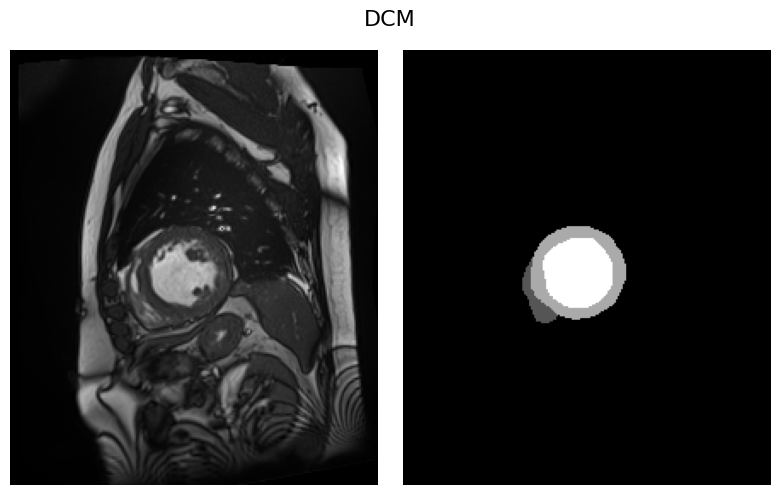
\includegraphics[width=0.65\textwidth]{figures/fig018.png}
    \caption*{Fonte: Autor}
    \label{fig:fig018}
\end{figure}

\begin{figure}[h!]
    \caption{Captura Diastólica de CMH}
    \centering
    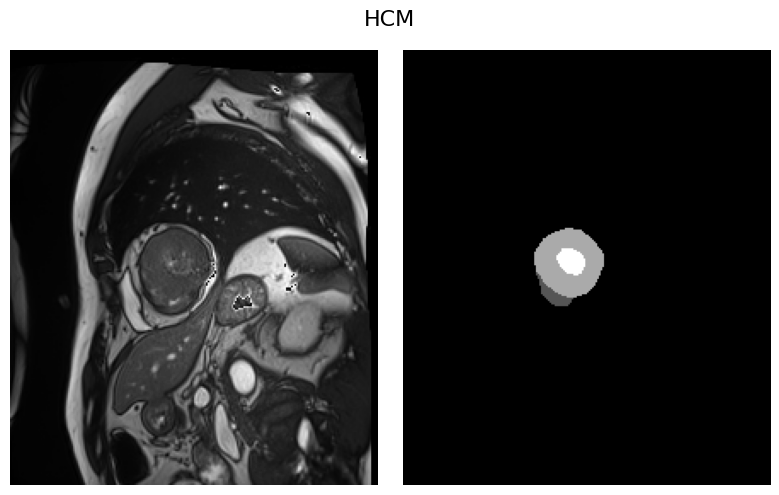
\includegraphics[width=0.65\textwidth]{figures/fig019.png}
    \caption*{Fonte: Autor}
    \label{fig:fig019}
\end{figure}

\begin{figure}[h!]
    \centering
    \caption{Captura Diastólica NOR}
    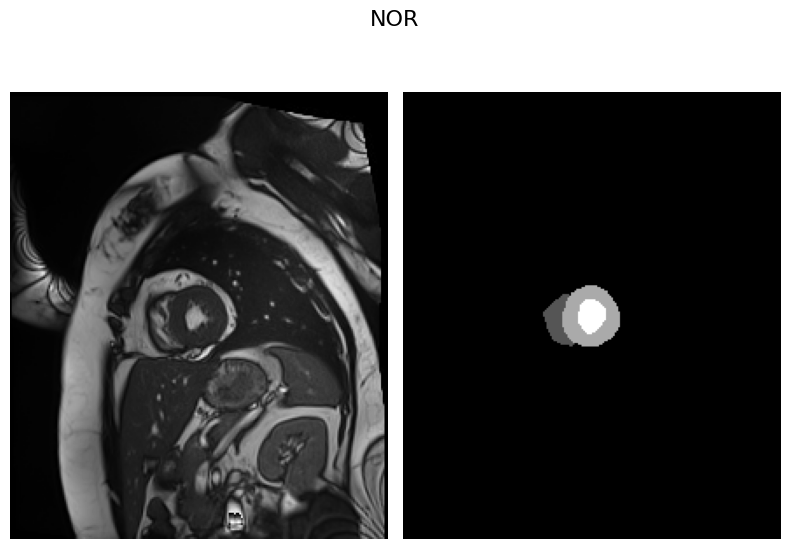
\includegraphics[width=0.65\textwidth]{figures/fig020.png}
    \caption*{Fonte: Autor}
    \label{fig:fig020}
\end{figure}

%--------------------------------------------------------
\subsection{RESULTADOS MODELO BASE}
\label{subsec:resultados_acdc_base}

Os resultados foram obtidos aplicando a metodologia previamente apresentada, foram extraídas as características radiômicas e profundas, após foi aplicado o \textit{F-Test} para seleção de características e o resultado concatenado na última dimensão, sendo $EMBED_{size} = 12$, o resultado é um vetor de características de $1\times24$. Em seguida, o modelo de autoatenção foi aplicado uma única vez conforma modelo original. Os hiperparâmetros utilizados são: taxa de aprendizado $\LR$, otimizador \gls{Adam}, tamanho de lote $\Batch$ e aproximadamente $\Epochs$ épocas. Por fim, é aplicada a função matemática sigmoide e definido o limite de $0,5$ para corte onde os valores acima deste limite são classificados como \gls{CMH} e os demais como normal. As métricas resultantes podem ser conferidas na Tabela \ref{tab:metrics}. A matriz de confusão é apresentada na Figura \ref{fig:fig016} e um gráfico ilustrando da \gls{ROC} é apresentado na Figura \ref{fig:fig017}.
\newline

\begin{table}[h!]
    \centering
    \caption{Métricas do Experimento - Modelo Base}
    \renewcommand{\arraystretch}{1} % default é 1 
    \begin{tabular}{|c|c|}
    \hline 
          \textbf{Métrica} & \textbf{Valor} \\ 
    \hline 
        Acurácia & 0.58 \\ 
    \hline 
        Precisão & 0.47 \\ 
    \hline 
        Revocação & 0.40 \\ 
    \hline 
        AUC & 0.55 \\ 
    \hline 
    \end{tabular} 
    \caption*{Fonte: Autor}
    \label{tab:metrics}
\end{table}

\begin{figure}[h!]
    \centering
    \caption{Matriz de Confusão -  Modelo Base}
    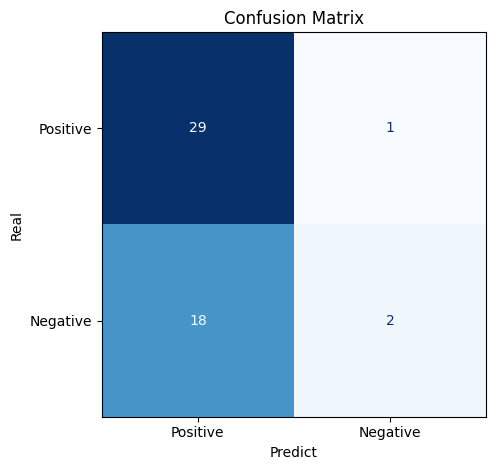
\includegraphics[width=0.55\textwidth]{figures/fig016.png}
    \caption*{Fonte: Autor}
    \label{fig:fig016}
\end{figure}

\begin{figure}[h!]
    \centering
    \caption{ROC}
    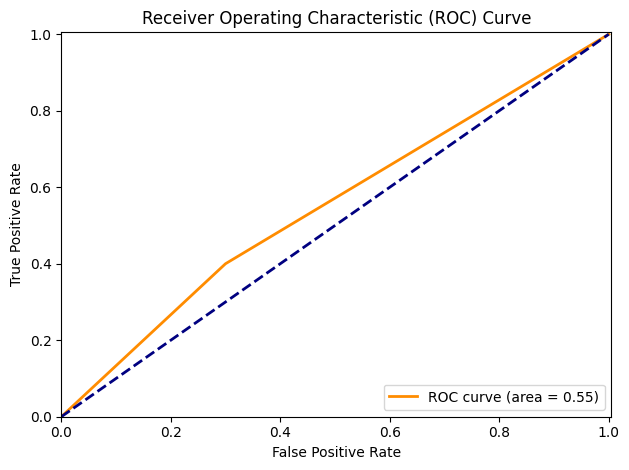
\includegraphics[width=0.75\textwidth]{figures/fig017.png}
    \caption*{Fonte: Autor}
    \label{fig:fig017}
\end{figure}


Para o registro dos resultados foi utilizado a ferramenta \textit{CometML}. O \textit{CometML} pode registrar, em tempo de execução, informações como erro por lote, erro por época, acurácia de validação, etc, podem ser armazenados enquanto o processo de treinamento é executado. Por fim métricas como acurácia e matriz de confusão podem ser geradas também.O serviço é acessado  por uma \gls{API} externa. As Figuras \ref{fig:fig028} e \ref{fig:fig029} demonstram respectivamente os painéis adaptáveis ao fim do treino e os valores armazenado de erro, acurácia, etc, coletados durante o treino.

\begin{figure}[h!]
    \centering
    \caption{Painéis Adaptáveis - \textit{CometML}}
    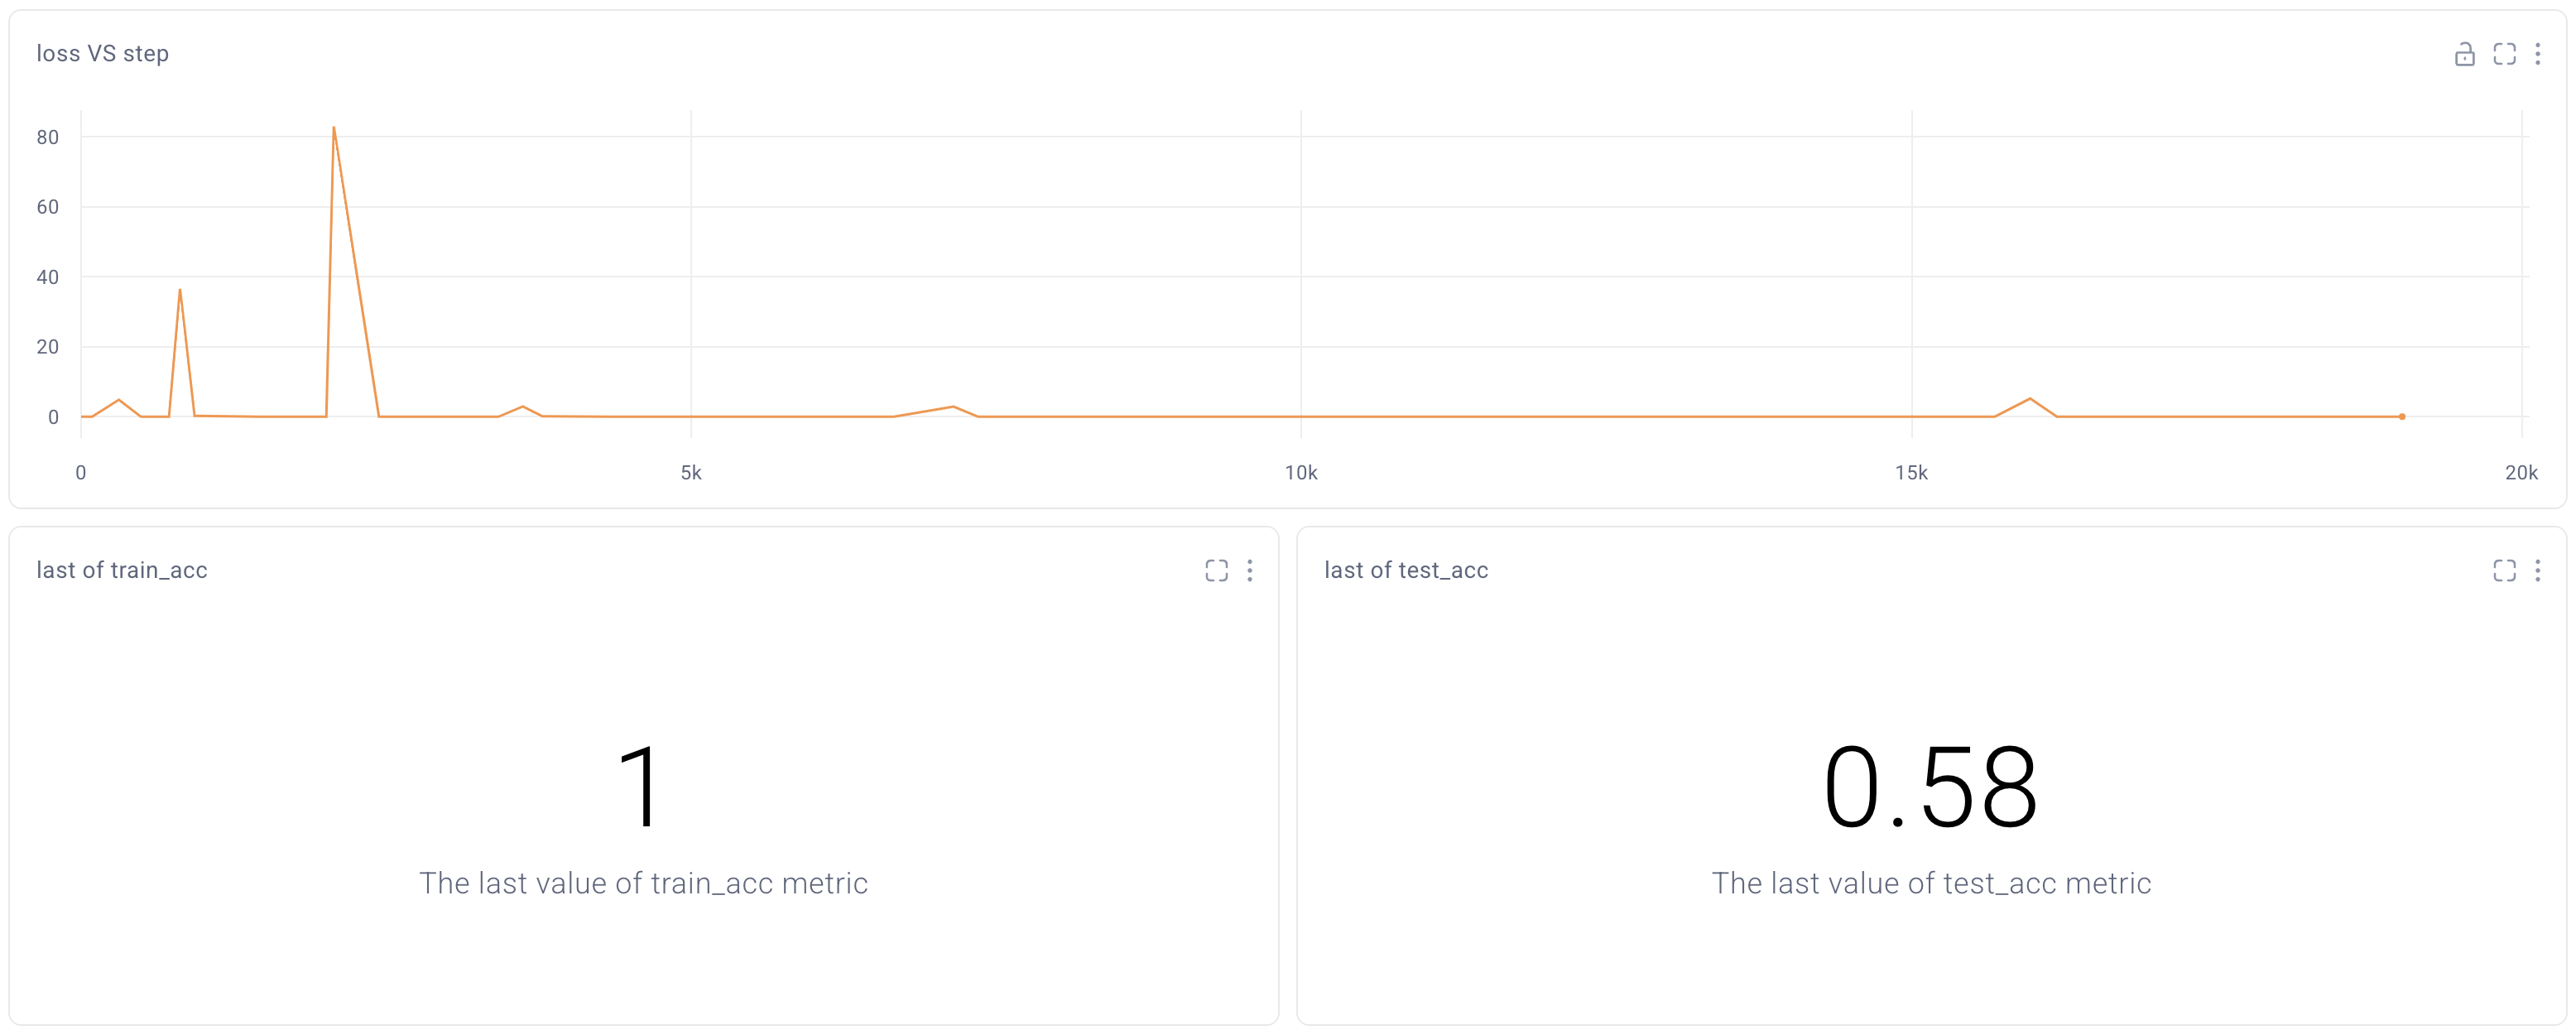
\includegraphics[width=1\textwidth]{figures/fig028.png}
    \caption*{Fonte: Autor}
    \label{fig:fig028}
\end{figure}


\begin{figure}[h!]
    \centering
    \caption{Valores Coletados no Treino - \textit{CometML}}
    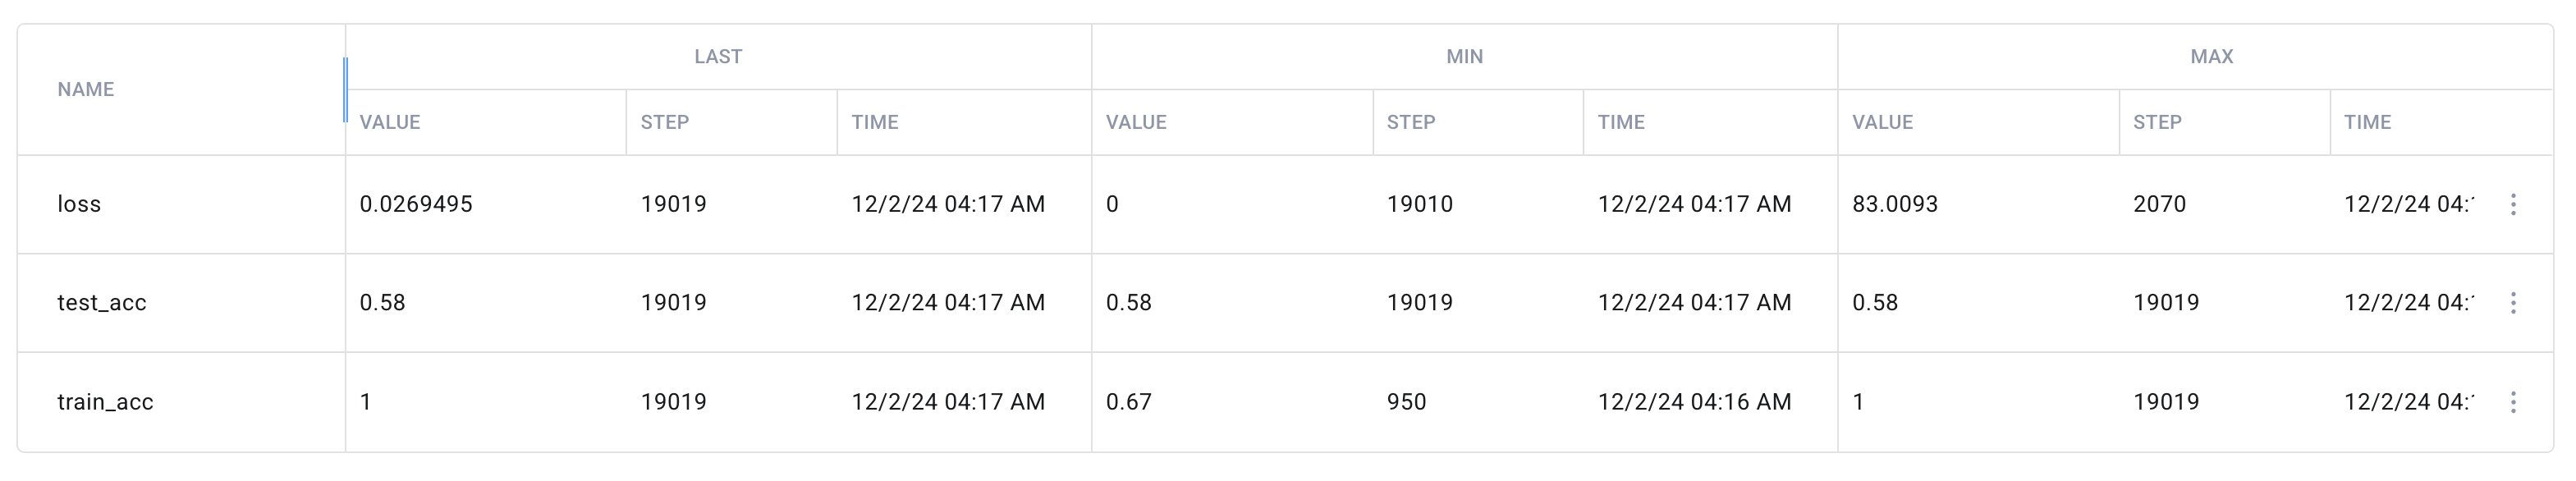
\includegraphics[width=1\textwidth]{figures/fig029.png}
    \caption*{Fonte: Autor}
    \label{fig:fig029}
\end{figure}


%--------------------------------------------------------
\subsection{RESULTADOS MODELOS ADAPTADOS}
\label{subsec:resultados_acdc_adaptado}

Preencher...

%--------------------------------------------------------
\section{Considerações Finais do Capítulo} 
\label{sec:cap6_consideracoes_finais}

Os resultados obtidos, aplicando a arquitetura proposta por \citeonline{aiSelfAttentionBasedFusion2023} com modificações na quantidade de características utilizadas e aplicado em imagens de \gls{RMC} para identificação de cardiomiopatias, em contraste com o trabalho mencionado que foi aplicado à identificação de câncer no pulmão, obteve resultados menos relevantes que o original. Isto indica que há espaço para exploração e melhorias a serem proposta para o âmbito de cardiomiopatia. Algumas, abordagens ainda são tidas em vista como manipular o seletor de características e a sua quantidade, testar novos hiperparâmetros para os modelos, ao invés de ter um único módulo de autoatenção, aplicar vários em cascata, etc.

